\newpage
\section{Podręcznik użytkownika}  %6
%Opis jak używać programu. Mogą być z zrzut ekranu razem z opisem. 
\subsection{Logowanie}

Po uruchomieniu aplikacji po raz pierwszy użytkownik zostanie przekierowany na ekran logowania. Należy wprowadzić adres e-mail oraz hasło, a następnie kliknąć przycisk \textbf{'Zaloguj' } \textbf{Rys. \ref{rys:ekranlogowania2} (s. \pageref{rys:ekranlogowania2})}.
\begin{figure}[h!]
	\centering
	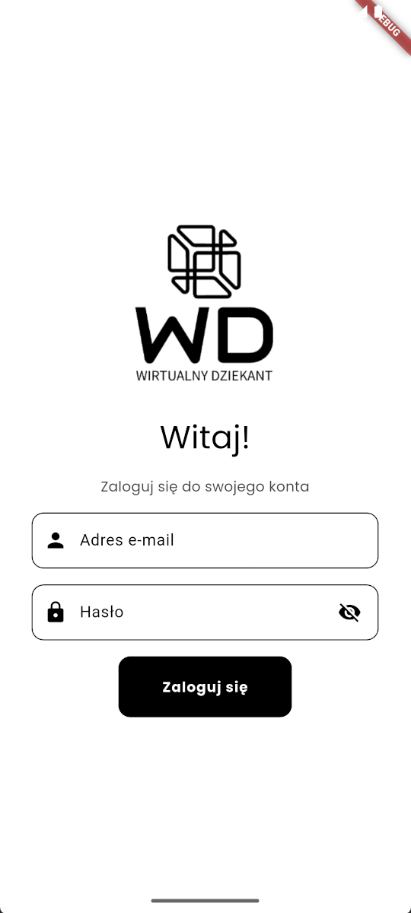
\includegraphics[width=0.5\textwidth]{rys/ekranlogowania.png}
	\caption{Ekran logowania}
	\label{rys:ekranlogowania2}
\end{figure}

\subsection{Ekran główny}

Po zalogowaniu użytkownik zostanie przekierowany na ekran główny. Na ekranie głównym znajduje się plan zajęć, który pokazuje nadchodzące zajęcia. Kliknięcie na konkretny dzień wyświetli szczegóły, takie jak sala, wykładowca i godziny. \textbf{Rys. \ref{rys:ekranglowny2} (s. \pageref{rys:ekranglowny2})}
\begin{figure}[h!]
	\centering
	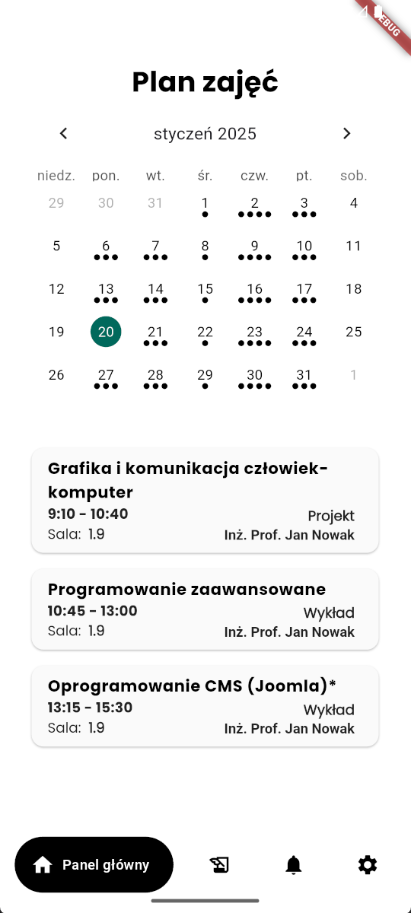
\includegraphics[width=0.5\textwidth]{rys/ekranplanzajec.png}
	\caption{Ekran główny}
	\label{rys:ekranglowny2}
\end{figure}


\newpage
\subsection{Przedmioty}
Aby zobaczyć jakie przedmioty mamy na danym semetrze należy kliknąć na ikonę Przedmioty. Na ekranie przedmioty znajduję się lista przedmitów jakie posiadamy w aktualnym semestrze, średnia ocen , oraz data zbliżających się egzaminów. \textbf{Rys. \ref{rys:Przedmiotyv3} (s. \pageref{rys:Przedmiotyv3})}
\begin{figure}[h!]
	\centering
	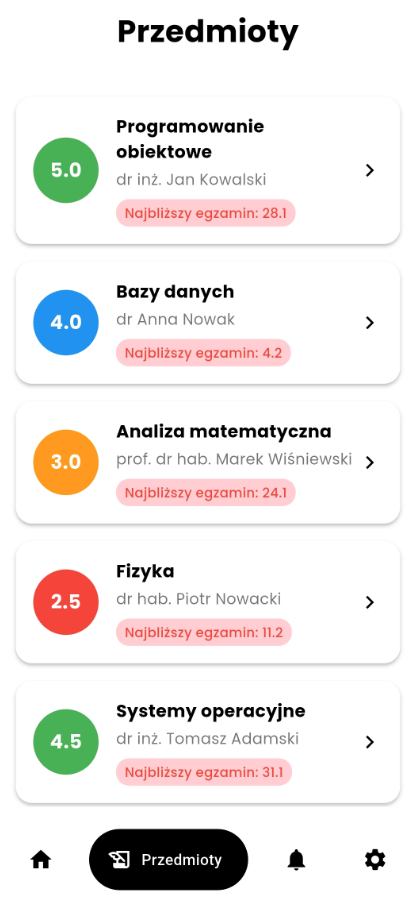
\includegraphics[width=0.55\textwidth]{rys/Przedmiotyv3.png}
	\caption{Ekran Przedmioty}
	\label{rys:Przedmiotyv3}
\end{figure}
\newpage
Jeżeli chcemy zobaczyć szczegóły danego przedmiotu (Np. wszystkie oceny). Nalęży kliknąć na szczałkę obok tego przedmiotu co poskutkuje przeniesieniem nas do jego szczegółów. \textbf{Rys. \ref{rys:Przedmiotyv4} (s. \pageref{rys:Przedmiotyv4})}
\begin{figure}[h!]
	\centering
	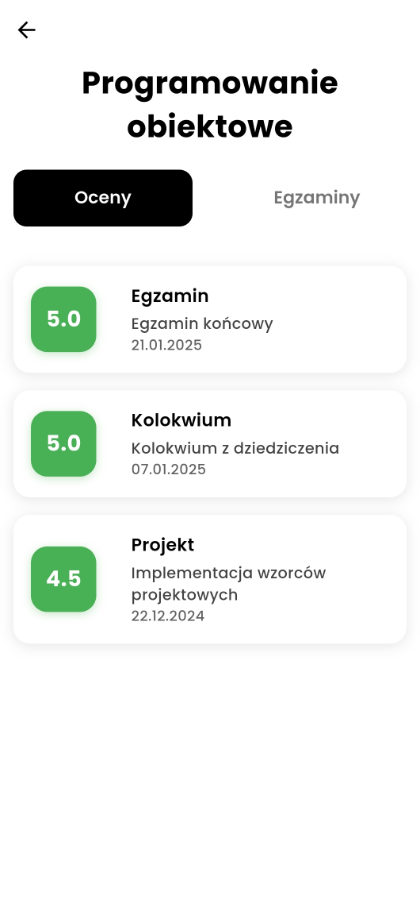
\includegraphics[width=0.55\textwidth]{rys/przedmiotyv4.png}
	\caption{Ekran szczegółowy dla danego Przedmiotu - Oceny}
	\label{rys:Przedmiotyv4}
\end{figure}
\newpage
Jeżeli chcielibyśmy przejść do szczegółów dotyczących Egzaminu dla danego przedmiotu należy kliknąć na okienko Egzaminy.  \textbf{Rys. \ref{rys:Przedmiotyv5} (s. \pageref{rys:Przedmiotyv5})}
\begin{figure}[h!]
	\centering
	
\includegraphics[width=0.55\textwidth]{rys/przedmiotyv5.png}
	\caption{Ekran szczegółowy dla danego Przedmiotu - Egzaminy}
	\label{rys:Przedmiotyv5}
\end{figure}

\newpage
\subsection{Ogłoszenia}

Aby zobaczyć ogłoszenia, należy kliknąć na ikonę Ogłoszenia w dolnym pasku nawigacyjnym. Po zrobieniu tego wyświetli się lista ogłoszeń. W zależności od ustawionego piorytetu danego ogłoszenia kolor boxa obok niego  będzię inny (Np. Pilne - Czerwony, Zwykłe - Szare). \textbf{Rys. \ref{rys:ekranpowiadomien} (s. \pageref{rys:ekranpowiadomien})}
\begin{figure}[h!]
	\centering
	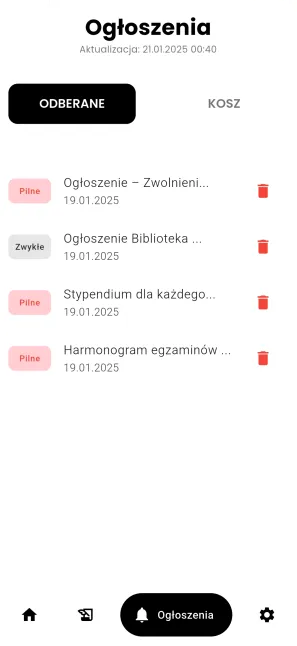
\includegraphics[width=0.5\textwidth]{rys/ekranpowiadomien.png}
	\caption{Ekran ogłoszeń}
	\label{rys:ekranpowiadomien}
\end{figure}
\newpage
Aby zobaczyć szczegóły danego ogłoszenie musimy je kliknąć. \textbf{Rys. \ref{rys:ogloszenieszcz} (s. \pageref{rys:ogloszenieszcz})}
\begin{figure}[h!]
	\centering
	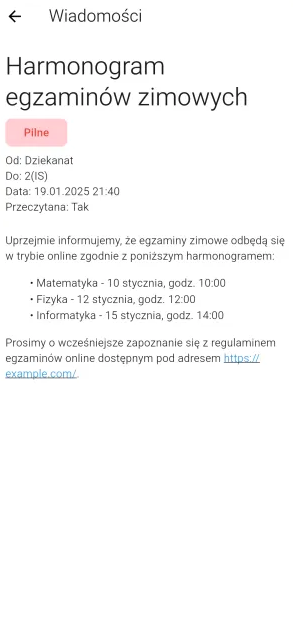
\includegraphics[width=0.55\textwidth]{rys/ogloszenieszcz.png}
	\caption{Szczegóły danego ogłoszenia}
	\label{rys:ogloszenieszcz}
\end{figure}
\newpage
Jeżeli na telefonie przyjdzie do nas powiadomie \textbf{Rys. \ref{rys:pushnot} (s. \pageref{rys:pushnot})}. To po kliknięciu na nie zostatniemy odrazu przekierowani do ekranu z ogłoszeniami \textbf{Rys. \ref{rys:pushnotv2} (s. \pageref{rys:pushnotv2})}.
\begin{figure}[h!]
	\centering
	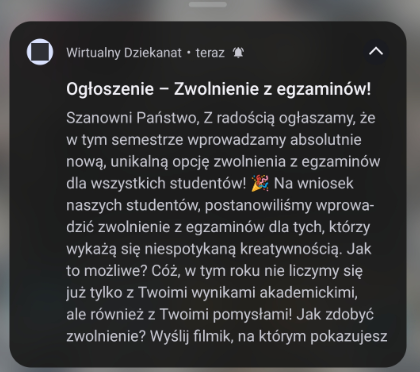
\includegraphics[width=0.7\textwidth]{rys/pushnot.png}
	\caption{Push notification}
	\label{rys:pushnot}
\end{figure}
\newpage
\begin{figure}[h!]
	\centering
	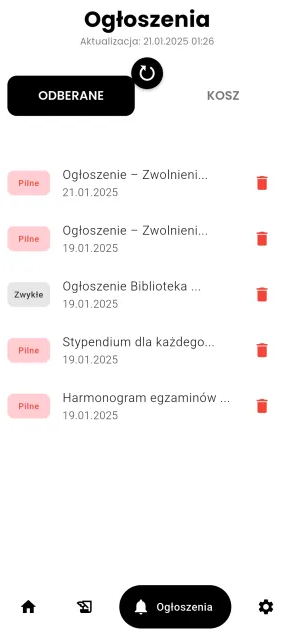
\includegraphics[width=0.6\textwidth]{rys/pushnotv2.png}
	\caption{Push notification}
	\label{rys:pushnotv2}
\end{figure}
\newpage

\subsection{Tryb offline - dostęp do zapisanych danych bez dostępu do Internetu}
\begin{figure}[htp!]
	\centering
	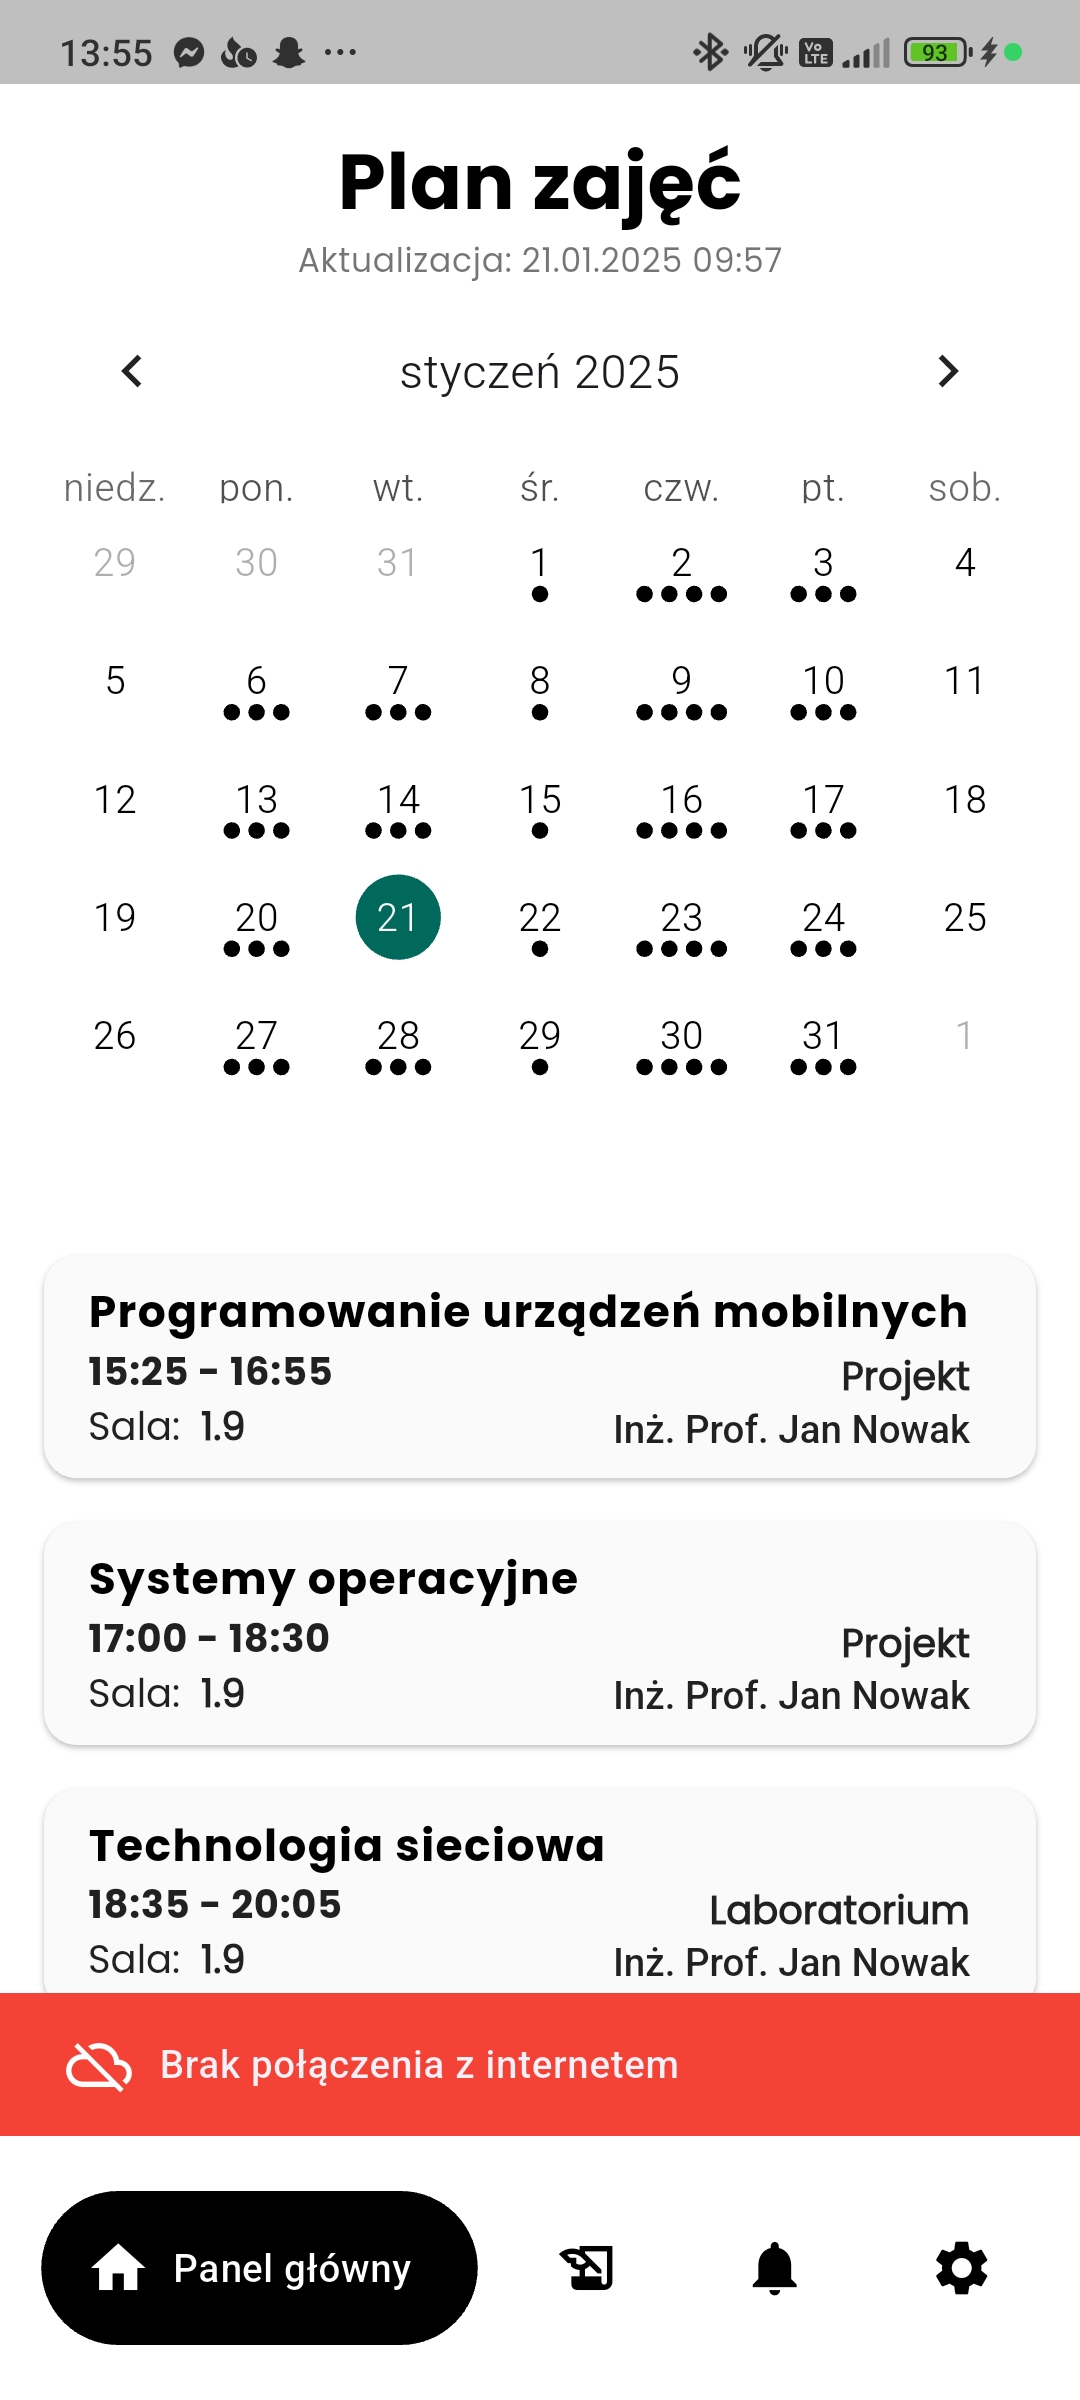
\includegraphics[width=0.6\textwidth]{rys/app_disconnected.jpg}
	\caption{Utracono połączenie z Internetem}
	\label{rys:pushnotv2}
\end{figure}
\newpage

\begin{figure}[htp!]
	\centering
	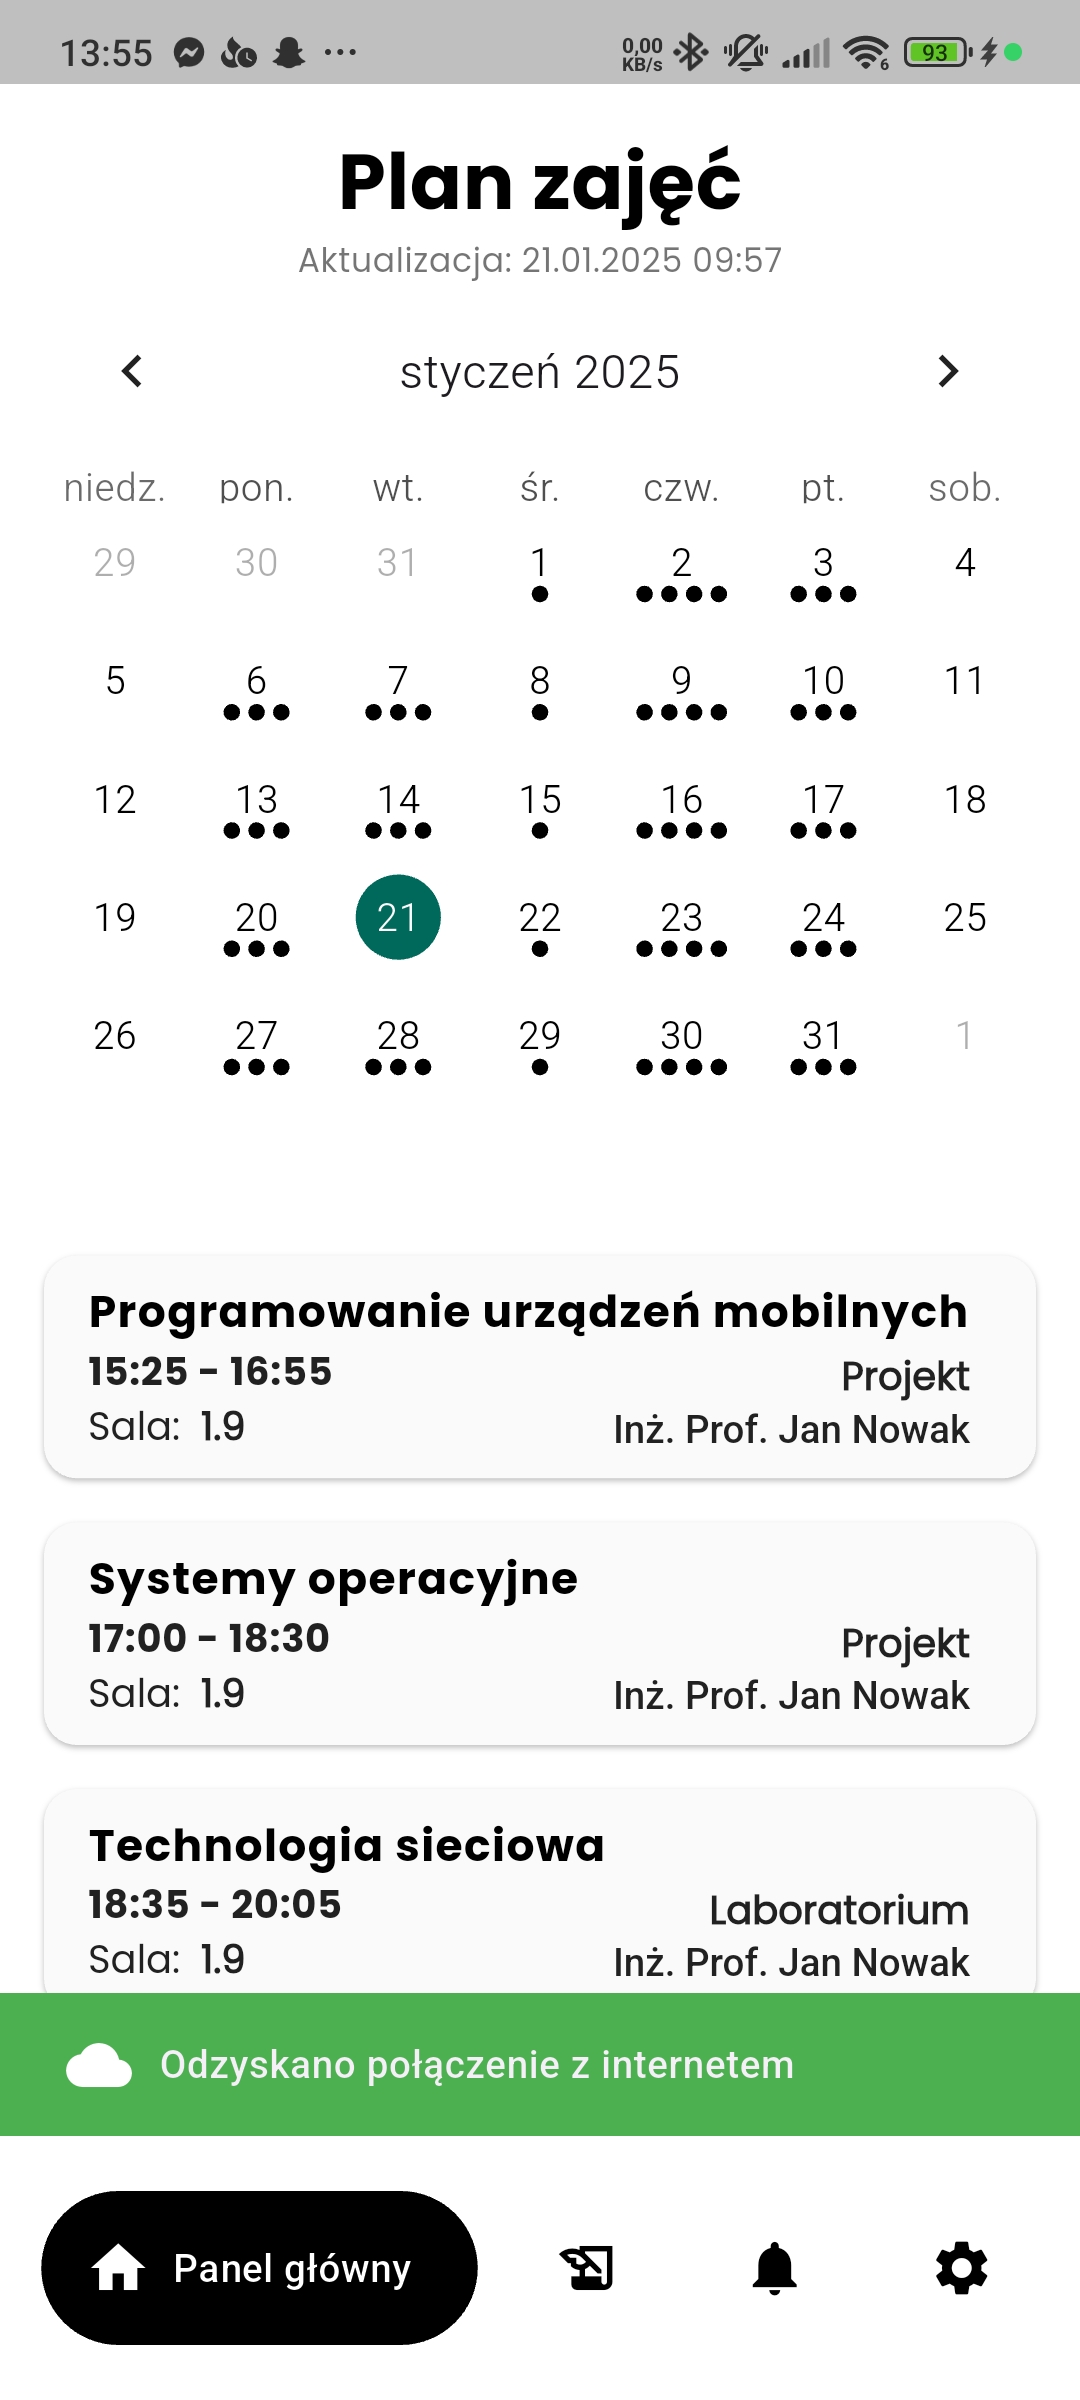
\includegraphics[width=0.6\textwidth]{rys/app_reconnected.jpg}
	\caption{Odzyskano połączenie z Internetem}
	\label{rys:pushnotv2}
\end{figure}

\newpage

\subsection{Ustawienia}

Aby przejść do ustawień, należy kliknąć na ikonę ustawień w dolnym pasku nawigacyjnym. W ustawieniach użytkownik może: \textbf{Rys. \ref{rys:ekranustawien1} (s. \pageref{rys:ekranustawien1})}

\begin{itemize}
	\item Włączyć lub wyłączyć tryb ciemny
	\item Zarządzać powiadomieniami
	\item Włączyć lub wyłączyć biometrię
\end{itemize}
\begin{figure}[htb!]
	\centering
	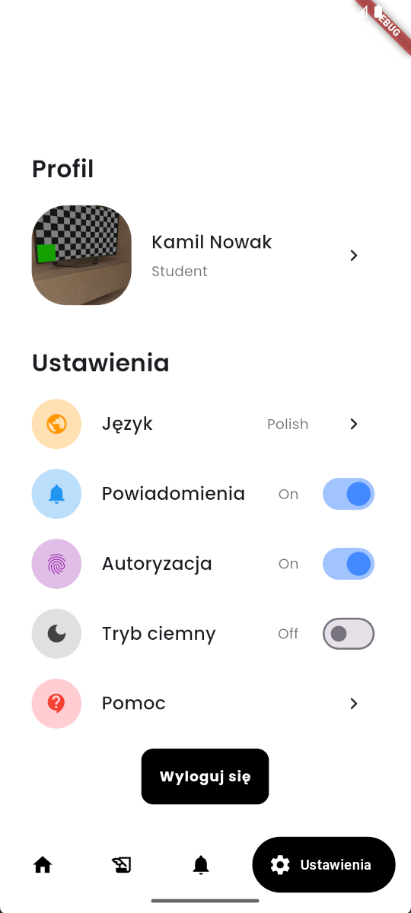
\includegraphics[width=0.5\textwidth]{rys/ekranustawien.png}
	\caption{Ekran ustawień}
	\label{rys:ekranustawien1}
\end{figure}
\newpage
\subsubsection{Tryb ciemny}

Aby włączyć tryb ciemny, należy przełączyć odpowiedni przełącznik w ustawieniach. Aplikacja automatycznie zmieni motyw na ciemny. \textbf{Rys. \ref{rys:darkmode} ,\ref{rys:whitemode}(s. \pageref{rys:darkmode} , \pageref{rys:whitemode})}
\\\textbf{DarkMode ON}:
\begin{figure}[h!]
	\centering
	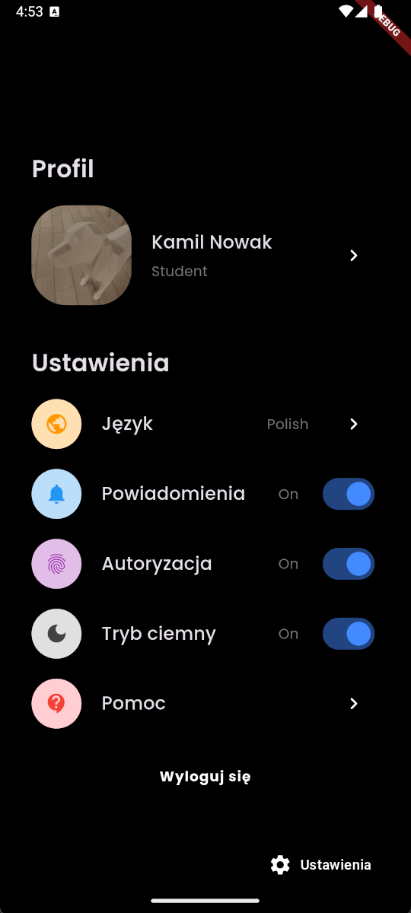
\includegraphics[width=0.55\textwidth]{rys/darkmode.png}
	\caption{Włączenie darkmoda}
	\label{rys:darkmode}
\end{figure}
\newpage
\textbf{DarkMode OFF}:
\begin{figure}[h!]
	\centering
	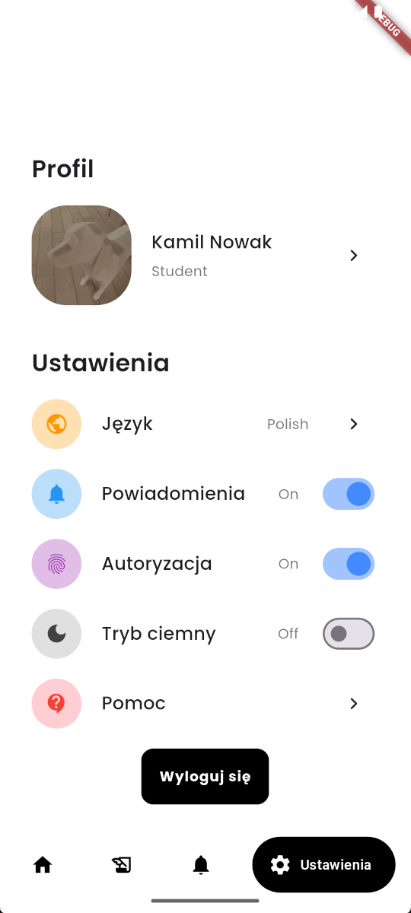
\includegraphics[width=0.55\textwidth]{rys/whitemode.png}
	\caption{Wyłączenie darkmoda}
	\label{rys:whitemode}
\end{figure}

\newpage
\subsubsection{Zarządzanie powiadomieniami}
W ustawieniach można włączyć lub wyłączyć powiadomienia dla różnych typów zdarzeń, takich jak nadchodzące zajęcia czy nowe oceny.\textbf{Rys. \ref{rys:notificationON}, \ref{rys:notificationOFF} (s. \pageref{rys:notificationON}, \pageref{rys:notificationOFF})}
\\\textbf{Powiadomienia ON:}
\begin{figure}[h!]
	\centering
	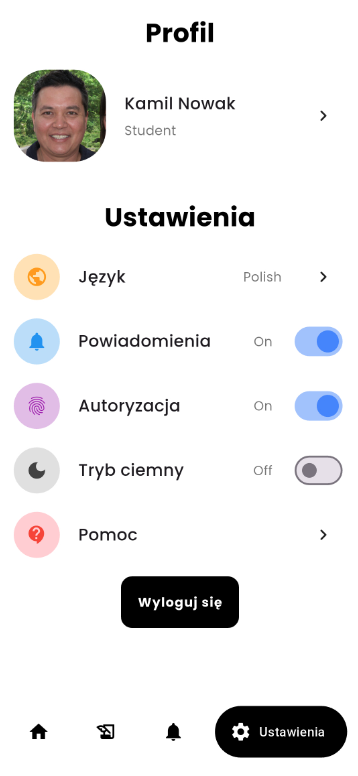
\includegraphics[width=0.55\textwidth]{rys/biometricssONN.png}
	\caption{Zarządzanie powiadomieniami ON}
	\label{rys:notificationON}
\end{figure}
\newpage
\textbf{Powiadomienia OFF:}
\begin{figure}[h!]
	\centering
	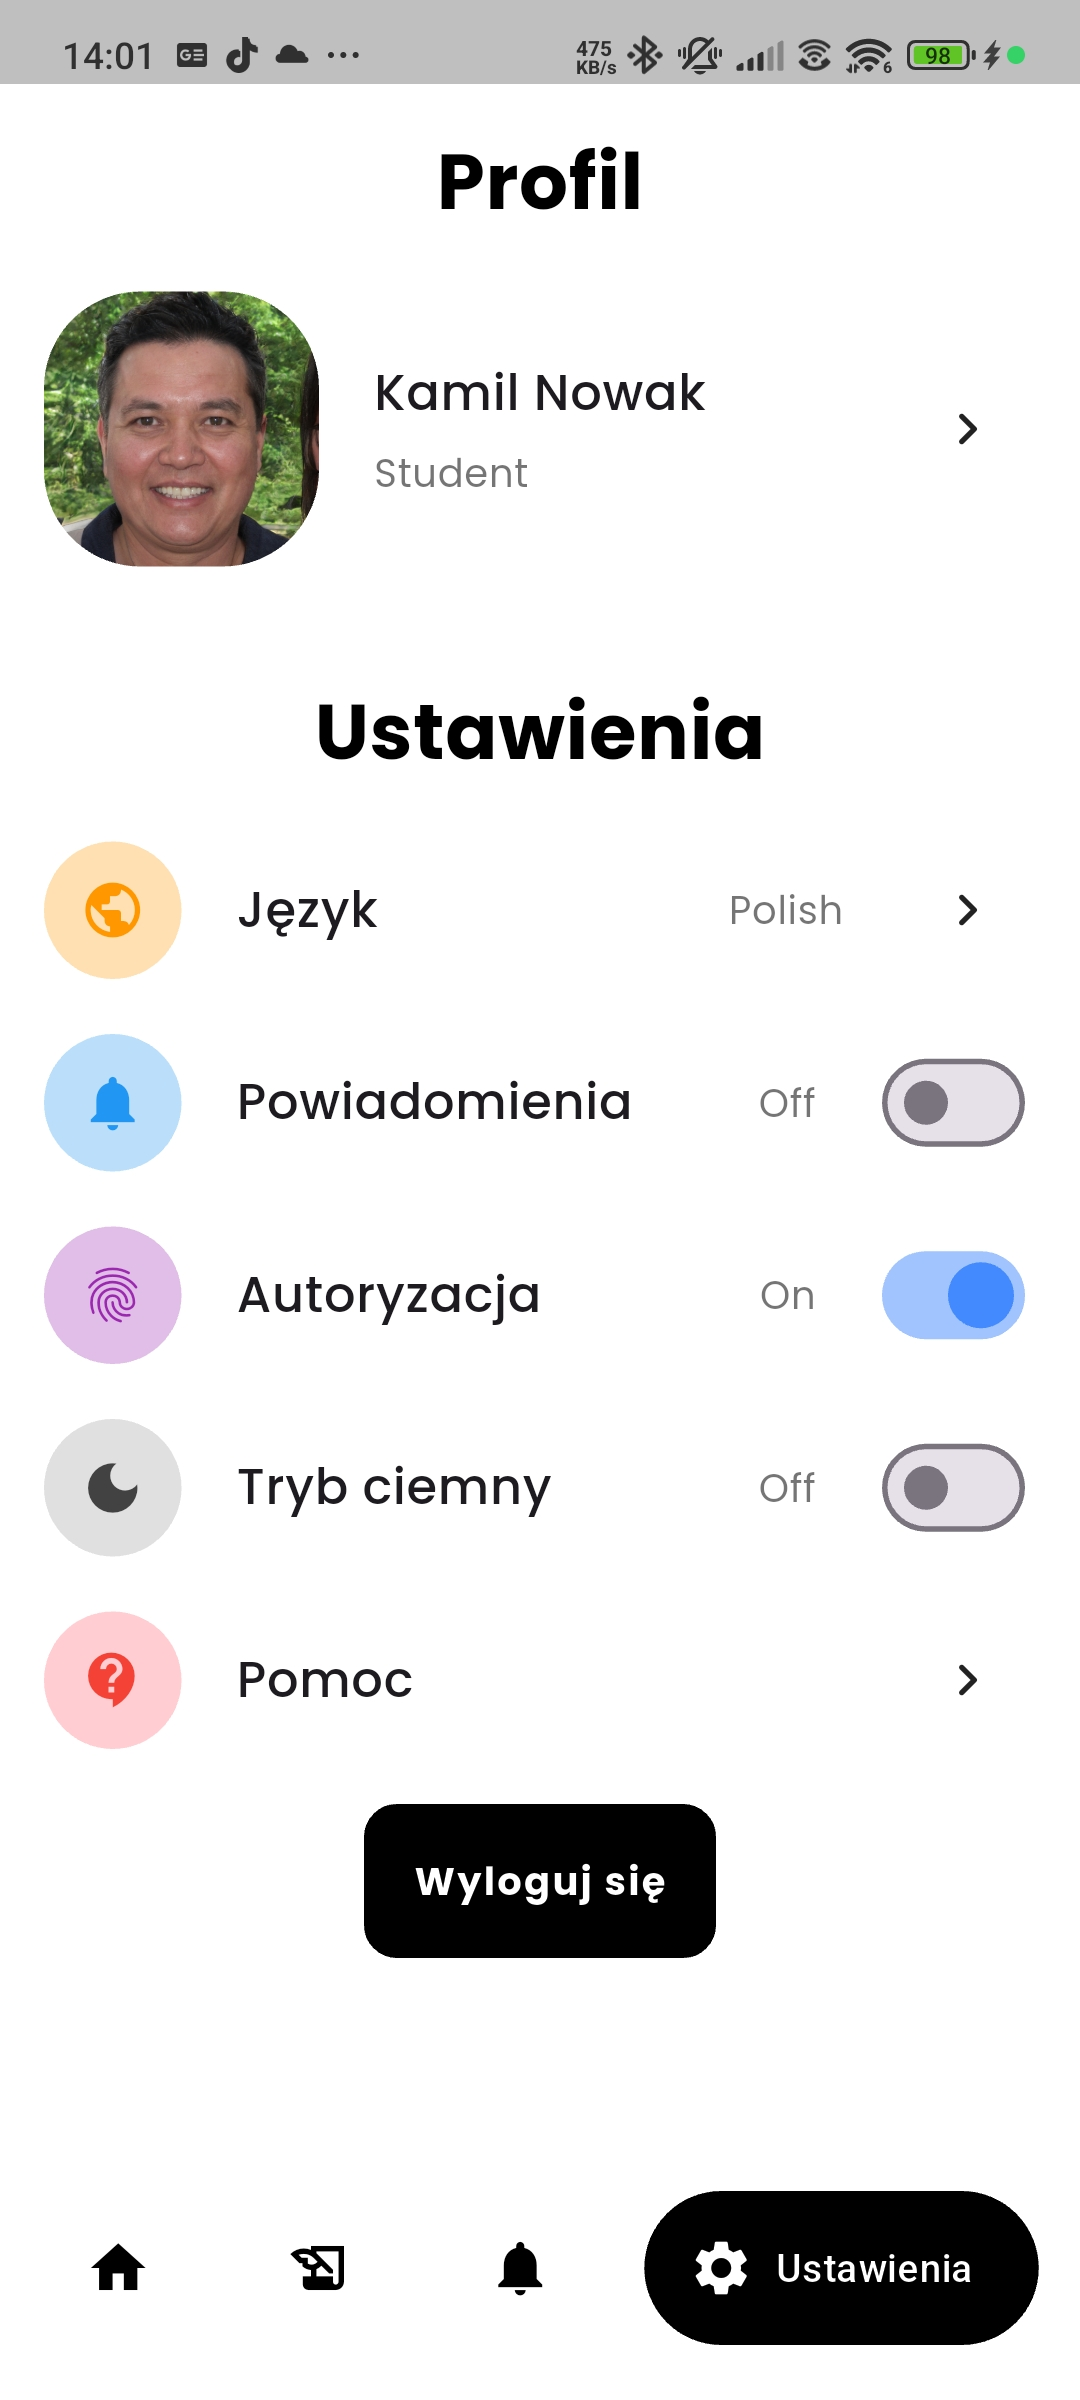
\includegraphics[width=0.55\textwidth]{rys/app_notifications_off.jpg}
	\caption{Zarządzanie powiadomieniami OFF}
	\label{rys:notificationOFF}
\end{figure}

\newpage
\subsubsection{Profil użytkownika}

Kliknięcie na avatar w ustawieniach przenosi użytkownika do ekranu profilu \textbf{Rys. \ref{rys:ekranustawien2} (s. \pageref{rys:ekranustawien2})}:, gdzie można
\begin{itemize}
	\item Zmienić zdjęcie profilowe
	\item Zobaczyć informacje o sobie, takie jak imię, nazwisko, adres e-mail
\end{itemize}
\begin{figure}[h!]
	\centering
	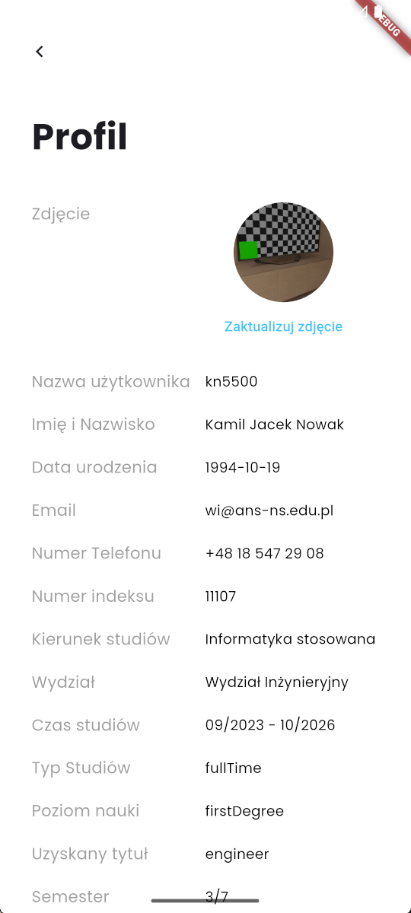
\includegraphics[width=0.5\textwidth]{rys/ekranustawienv2.png}
	\caption{Ekran ustawień}
	\label{rys:ekranustawien2}
\end{figure}
\newpage
Aby zaktualizować zdjęcie należy kliknąć na przycisk \textbf{`Zaktualizuj Zdjęcie`}.Po kliknięciu mamy do wyboru 2 opcje (Wybierz z galerii, Zrób zdjęcie) \textbf{Rys. \ref{rys:ekranustawienv3} (s. \pageref{rys:ekranustawienv3})}
\begin{figure}[h!]
	\centering
	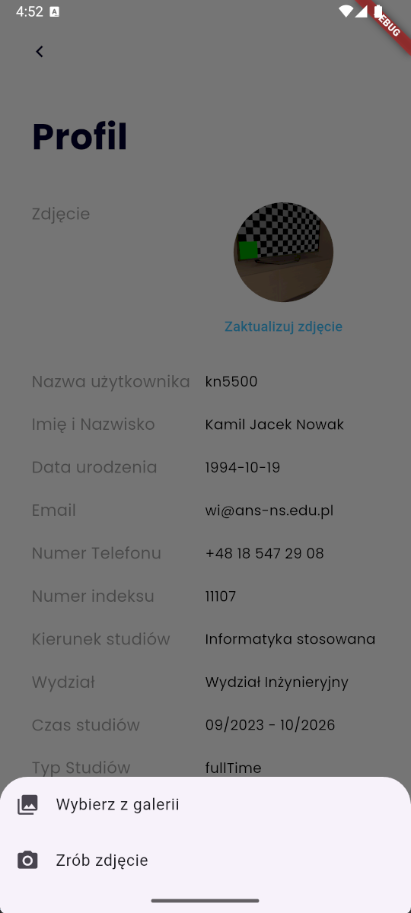
\includegraphics[width=0.55\textwidth]{rys/ekranustawienv3.png}
	\caption{Wybór aktualizacji zdjęcia}
	\label{rys:ekranustawienv3}
\end{figure}
\newpage
Po zrobieniu zdjęcia Gdy wyszstko przebiegło pomyślnie powienien wyświetlić się zielony komunikat "Zdjęcie zostało zaktualizowane" co oznacza że zostało pomyślnie zaktualizowane w naszej bazy danych.  \textbf{Rys. \ref{rys:ekranustawienv4} (s. \pageref{rys:ekranustawienv4})}
\begin{figure}[h!]
	\centering
	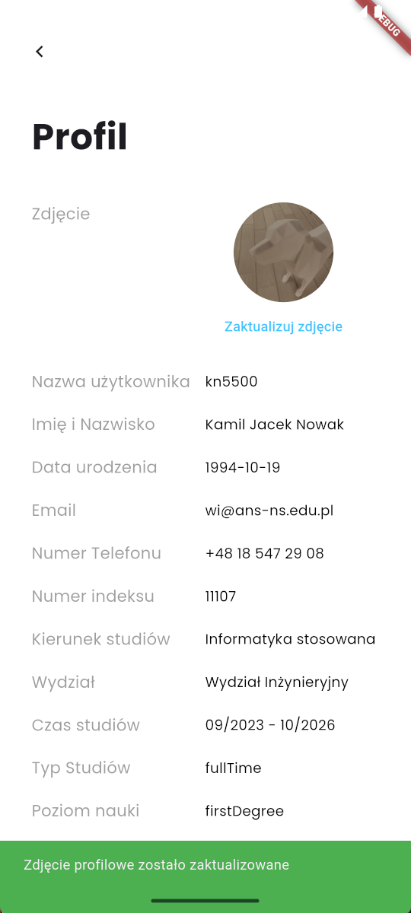
\includegraphics[width=0.55\textwidth]{rys/ekranustawienv4.png}
	\caption{Zdjęcie zostało poprawnie zrobione i do naszej bazy dancyh}
	\label{rys:ekranustawienv4}
\end{figure}
\newpage
\subsubsection{Biometria}
Po restracie apliakcji biometria pozwala na automatyczne logowanie się wcześniejszymi danymi poprzez odcisk palca przez co nie musimy na nowo wpisywać naszych danych.
\\Biomteria OFF \textbf{Rys. \ref{rys:biomteriaOFF} (s. \pageref{rys:biomteriaOFF})}:
\begin{figure}[h!]
	\centering
	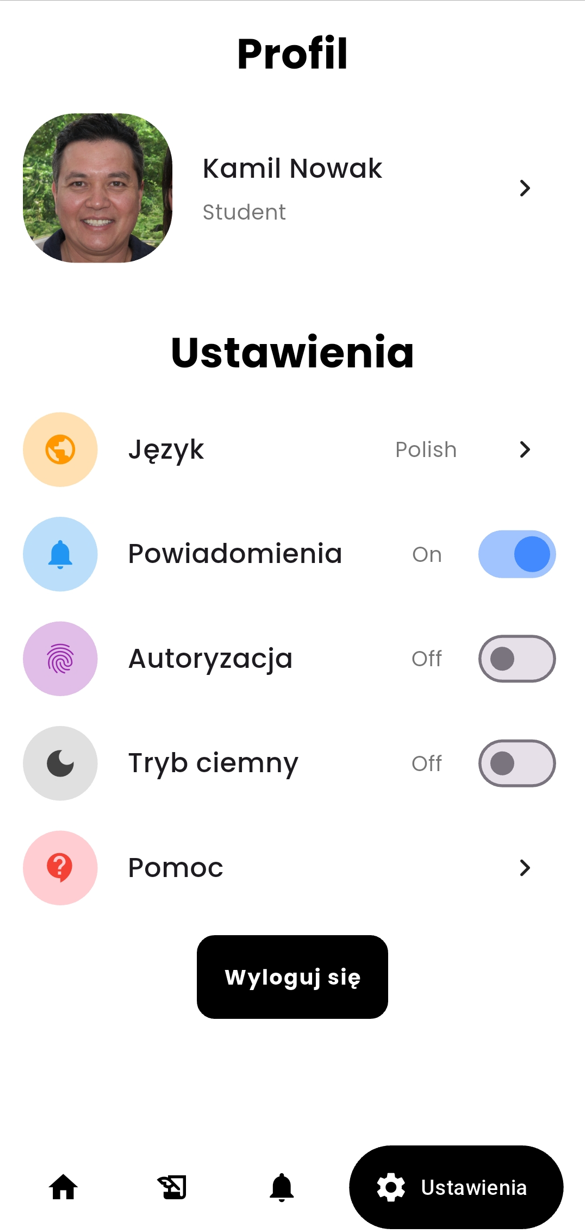
\includegraphics[width=0.55\textwidth]{rys/biometrics_off.png}
	\caption{Biomteria OFF}
	\label{rys:biomteriaOFF}
\end{figure}
\newpage
Biomteria ON \textbf{Rys. \ref{rys:biomteriaON} (s. \pageref{rys:biomteriaON})}:
\begin{figure}[h!]
	\centering
	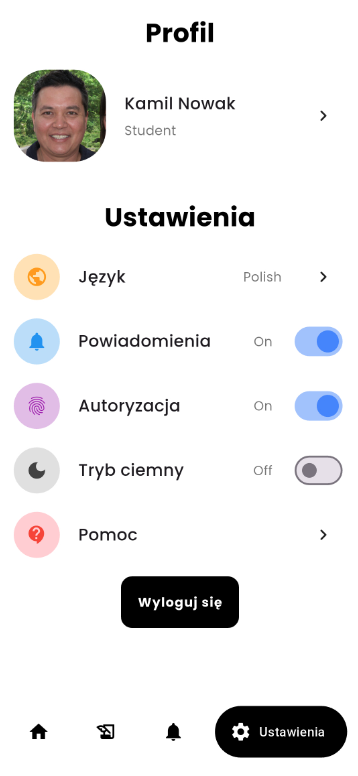
\includegraphics[width=0.55\textwidth]{rys/biometricssONN.png}
	\caption{Biometria ON}
	\label{rys:biomteriaON}
\end{figure}

\newpage
Gdy mamy włączoną biomterię to po wyłączeniu i właczeniu na nowo apikacji ta poprosi nas o podanie odcisku palca. Należy przyłożyć palec. Gdy weryfikacje się powiedzie to przeniesie nas do wnętrza aplikacji \textbf{Rys. \ref{rys:biomteriaON2} (s. \pageref{rys:biomteriaON2})}:
\begin{figure}[h!]
	\centering
	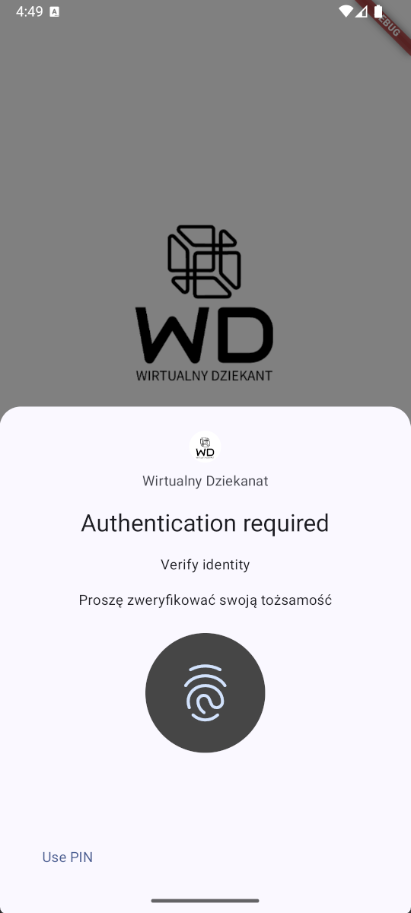
\includegraphics[width=0.55\textwidth]{rys/biometericON2.png}
	\caption{Poproszenie użytkownika o podanie odcisku palca}
	\label{rys:biomteriaON2}
\end{figure}

\newpage
\subsubsection{Wylogowanie}

Aby się wylogować, należy kliknąć na przycisk "Wyloguj się" na ekranie profilu. Użytkownik zostanie wylogowany i przekierowany na ekran logowania. \textbf{Rys. \ref{rys:wylogowanie} (s. \pageref{rys:wylogowanie})}

\begin{figure}[h!]
	\centering
	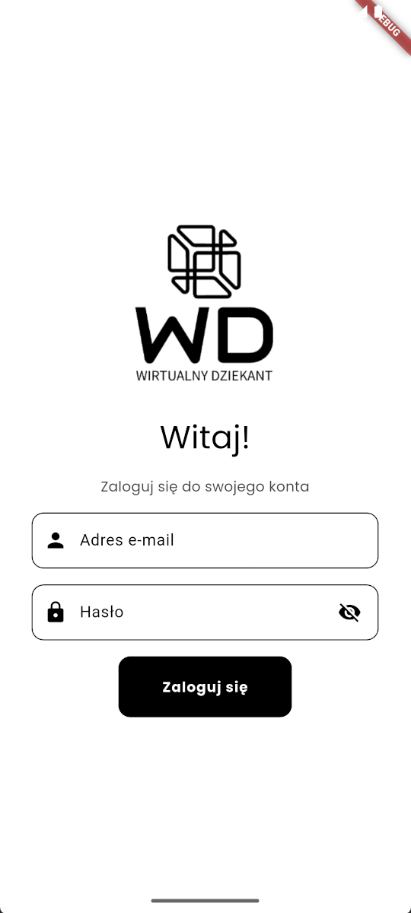
\includegraphics[width=0.6\textwidth]{rys/ekranlogowania.png}
	\caption{Widok po wylogowaniu}
	\label{rys:wylogowanie}
\end{figure}
\newpage
\subsection{Pull to refresh}
Aby użyć funkcji \textbf{pull to refresh} np. w panelu głównym musimy zrobić ruch palcem z góry aplikacji do środka (Powinno się utworzyć takie małe koło). Gdy już mamy palec na środku należy go puścić przez co naszę dane się automatycznie odświeżą. \textbf{Rys. \ref{rys:pull} (s. \pageref{rys:pull})}

\begin{figure}[h!]
	\centering
	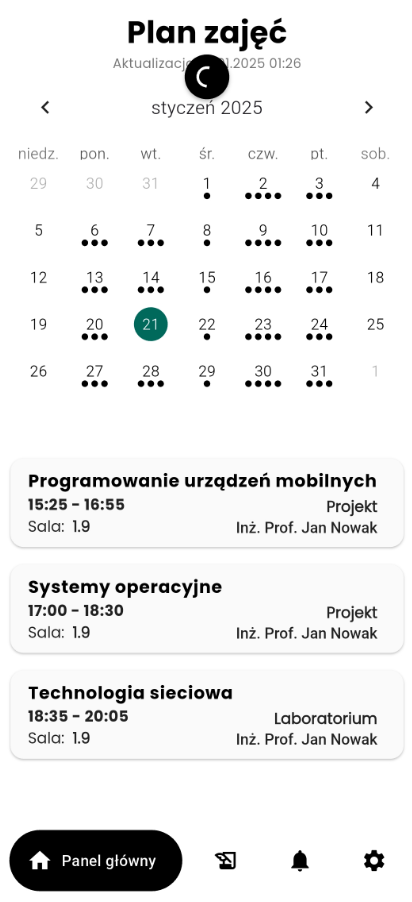
\includegraphics[width=0.55\textwidth]{rys/pull.png}
	\caption{Użycie pull to refresh}
	\label{rys:pull}
\end{figure}

\newpage
\subsection{Obsługa backendu}
Aby zalogować się do panelu administracyjnego backendu, należy przejść na stronę logowania i wprowadzić swoje dane uwierzytelniające. Po zalogowaniu użytkownik zostanie przekierowany do głównego interfejsu użytkownika, gdzie można zarządzać danymi aplikacji. \textbf{Rys. \ref{rys:be-login} (s. \pageref{rys:be-login})}

\begin{figure}[htp!]
	\centering
	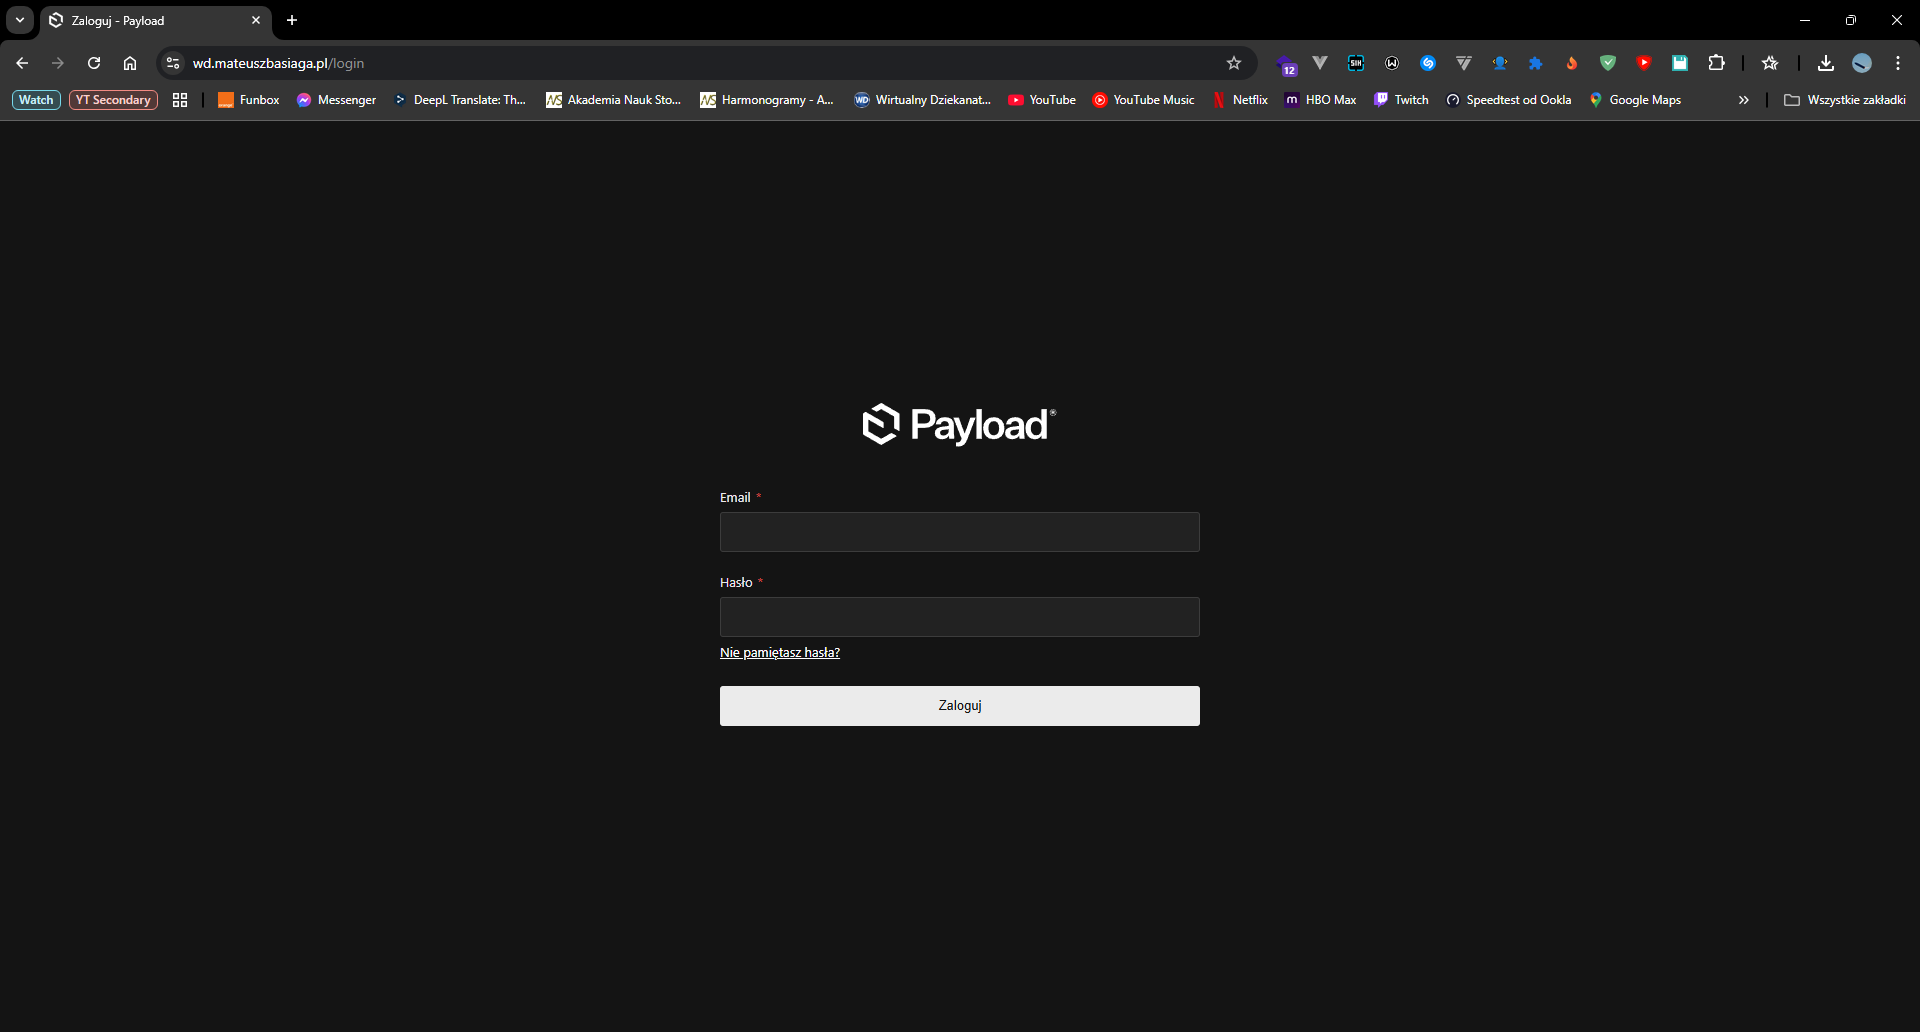
\includegraphics[width=\textwidth]{rys/be-login.png}
	\caption{Ekran logowania}
	\label{rys:be-login}
\end{figure}
\newpage
Główny interfejs użytkownika pozwala na przeglądanie i edytowanie danych, takich jak profile studentów, plan zajęć, ogłoszenia i inne. Użytkownik może również dodawać nowe wpisy oraz usuwać istniejące. \textbf{Rys. \ref{rys:be-main} (s. \pageref{rys:be-main})}

\begin{figure}[htp!]
	\centering
	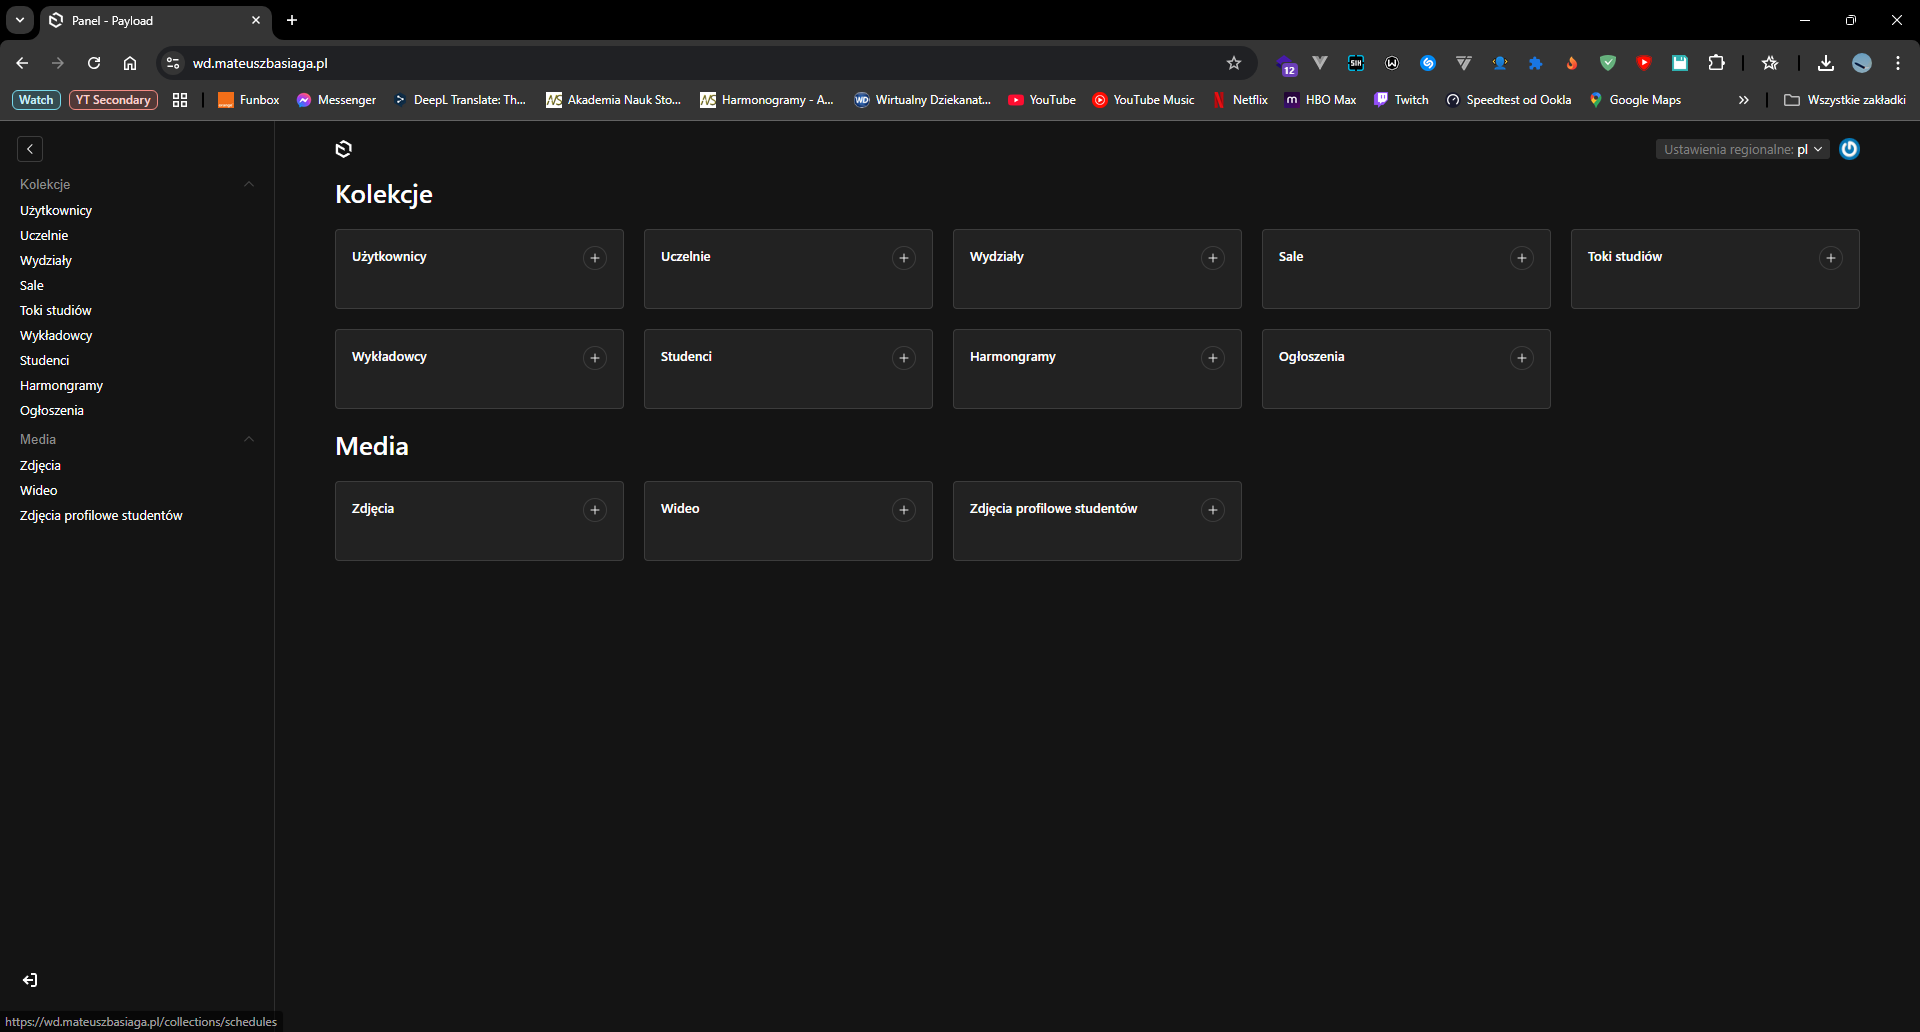
\includegraphics[width=\textwidth]{rys/be-main.png}
	\caption{Widok głównego interfejsu użytkownika}
	\label{rys:be-main}
\end{figure}

Profil studenta zawiera szczegółowe informacje o danym studencie, takie jak imię, nazwisko, adres e-mail, numer indeksu, rocznik, oceny i inne. Administrator może edytować te dane oraz dodawać nowe wpisy. \textbf{Rys. \ref{rys:be-student-profile} (s. \pageref{rys:be-student-profile})}

\begin{figure}[htp!]
	\centering
	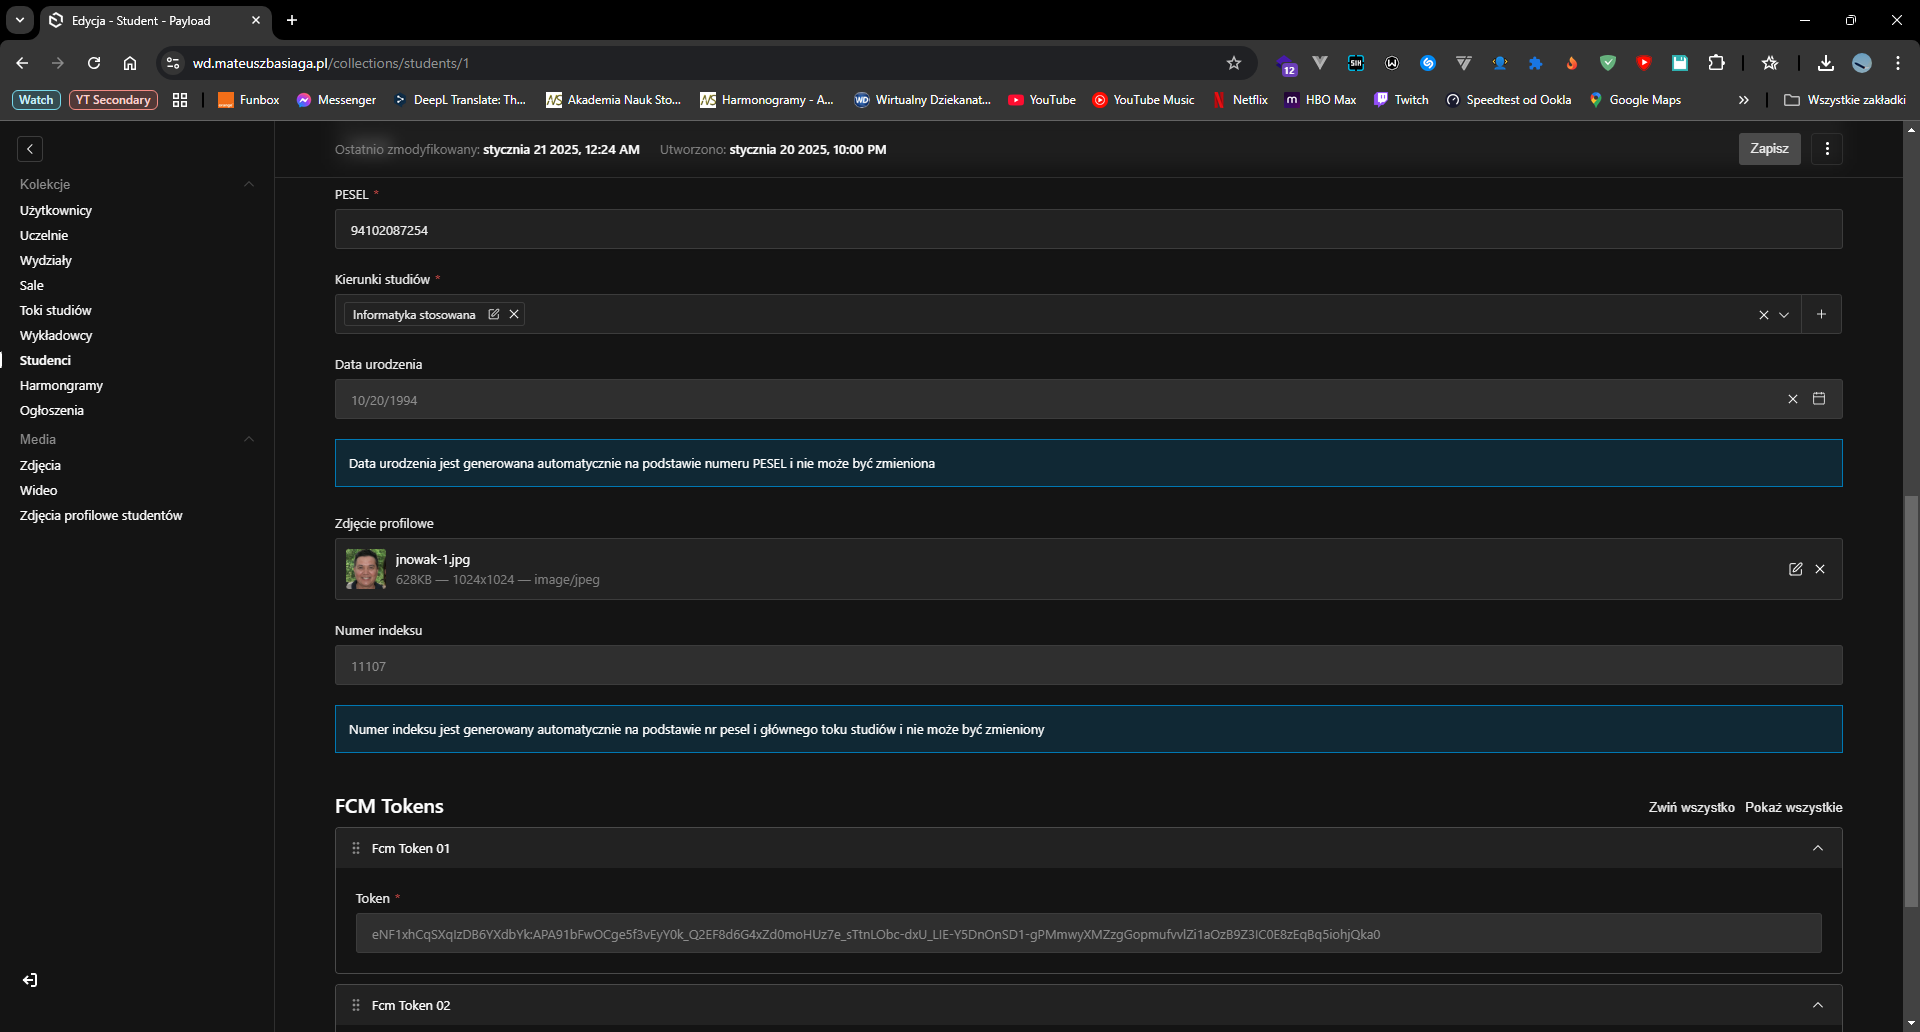
\includegraphics[width=\textwidth]{rys/be-student.png}
	\caption{Widok profilu studenta}
	\label{rys:be-student-profile}
\end{figure}
\newpage
Backend umożliwia również zarządzanie zdjęciami profilowymi studentów oraz innymi danymi multimedialnymi. Administrator może dodawać, edytować i usuwać zdjęcia profilowe. \textbf{Rys. \ref{rys:be-student-profi-pics} (s. \pageref{rys:be-student-profi-pics})}

\begin{figure}[htp!]
	\centering
	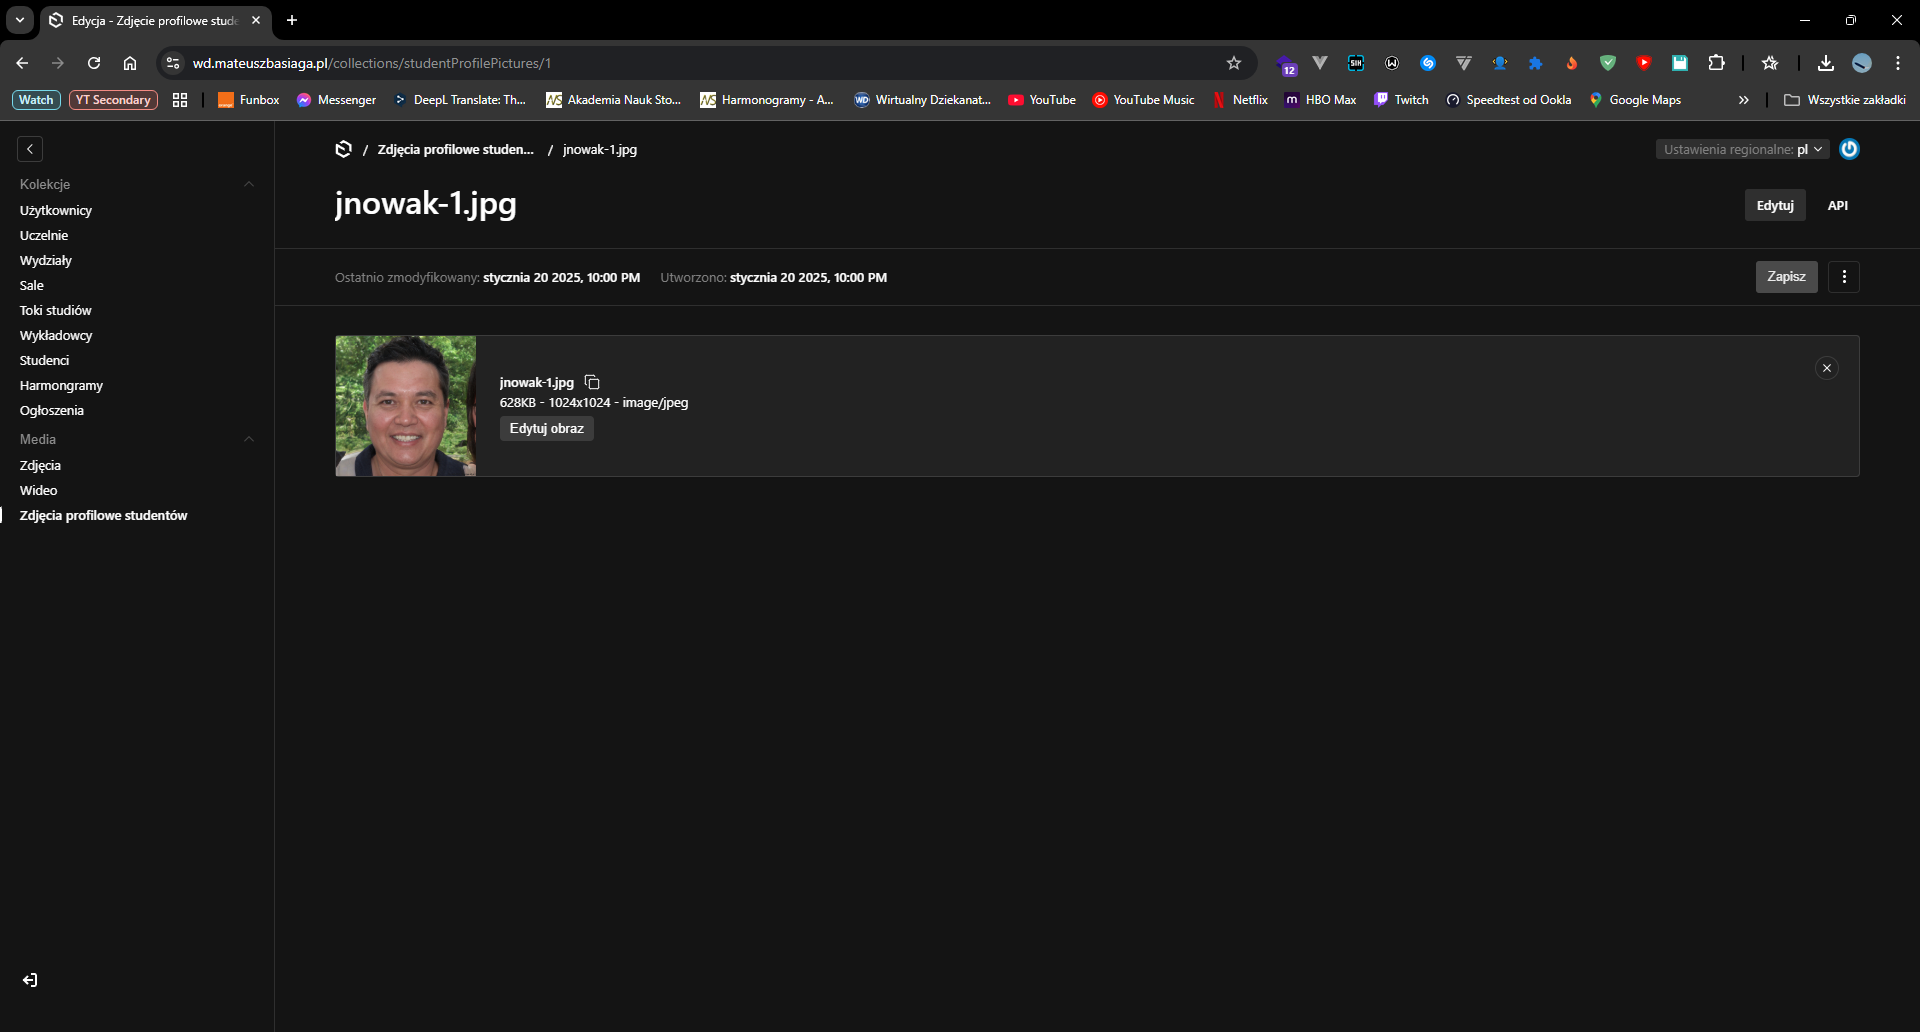
\includegraphics[width=\textwidth]{rys/be-student-prof-picture.png}
	\caption{Zdjęcia profilowe studentów - przykład danych multimedialnych}
	\label{rys:be-student-profi-pics}
\end{figure}

Plan zajęć można przeglądać i edytować za pomocą interfejsu backendu. Administrator może dodawać nowe zajęcia, edytować istniejące oraz usuwać wpisy. Plan zajęć jest synchronizowany z aplikacją mobilną, dzięki czemu studenci mają zawsze aktualne informacje. \textbf{Rys. \ref{rys:be-schedule} (s. \pageref{rys:be-schedule})}

\begin{figure}[htp!]
	\centering
	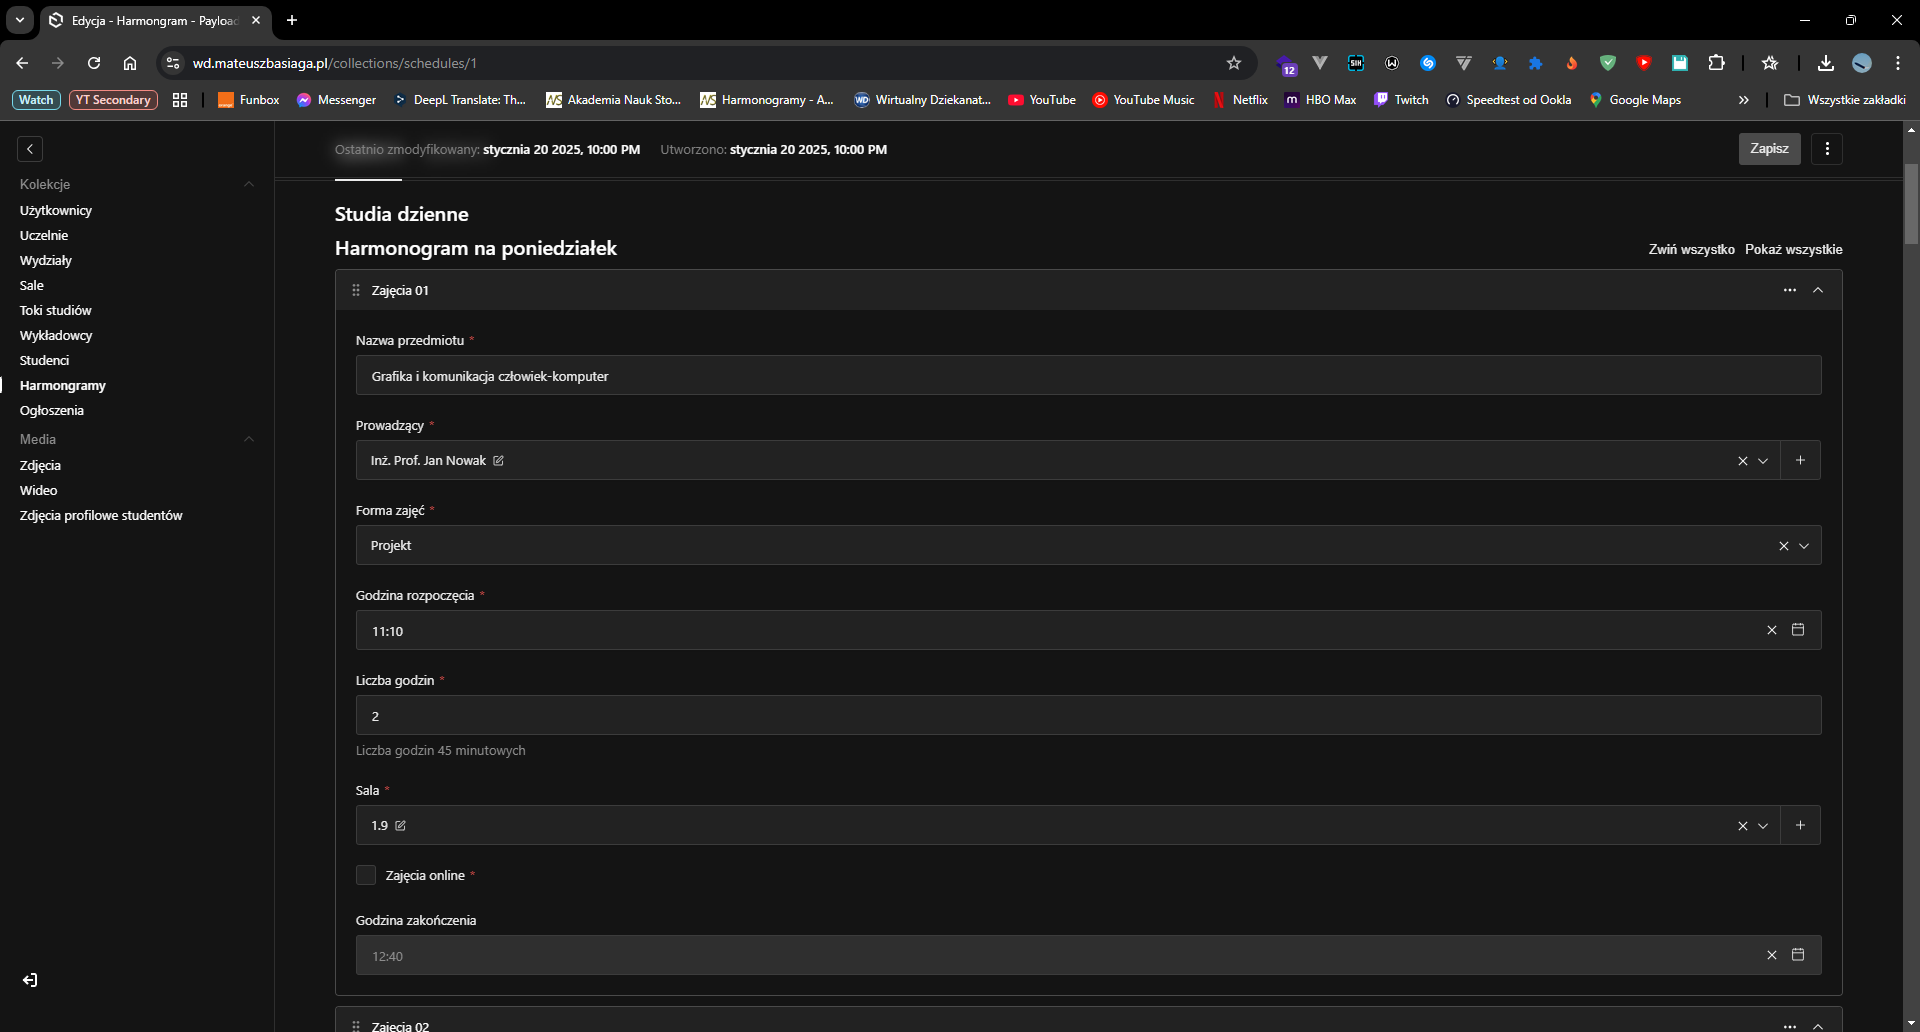
\includegraphics[width=\textwidth]{rys/be-schedule.png}
	\caption{Widok planu zajęć toku studiów}
	\label{rys:be-schedule}
\end{figure}
\newpage
Ogłoszenia można zarządzać za pomocą interfejsu backendu. Administrator może dodawać nowe ogłoszenia, edytować istniejące oraz usuwać wpisy. Ogłoszenia są synchronizowane z aplikacją mobilną, dzięki czemu studenci są na bieżąco informowani o ważnych wydarzeniach. \textbf{Rys. \ref{rys:be-announcement} (s. \pageref{rys:be-announcement})}

\begin{figure}[htp!]
	\centering
	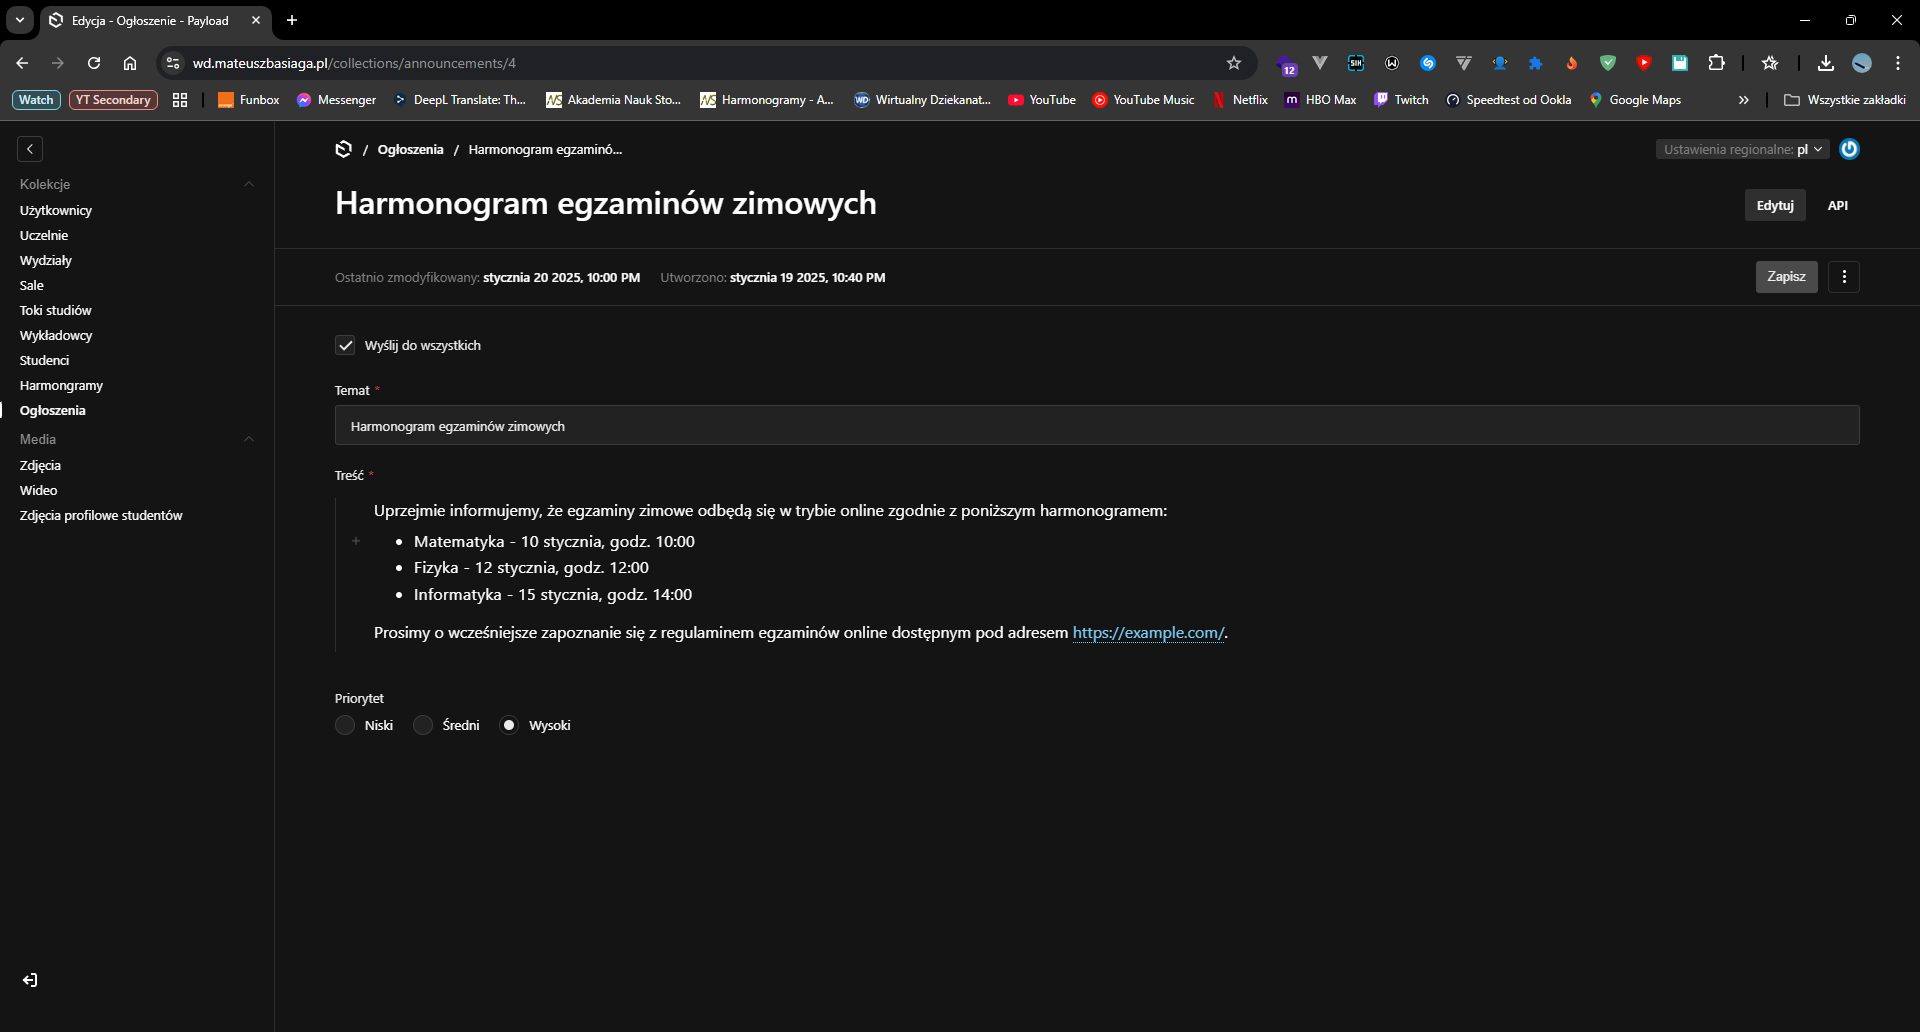
\includegraphics[width=\textwidth]{rys/be-announcement.png}
	\caption{Widok ogłoszenia}
	\label{rys:be-announcement}
\end{figure}

\nocite{www1}
\nocite{www2}
\nocite{www3}
\nocite{www4}
\nocite{www5}
\nocite{www6}
\nocite{www7}
\nocite{www8}
\nocite{www9}
\nocite{www10}
\nocite{www11}
\nocite{www12}
